This section provides the reader with an overview of Beverage Management. Beverage Management is an Android 
application that manages the beverages which a user has stored in their storage space. the application will have access
to a dataset of various drinks (beers in the initial release) and have will be able to populate the virtual storage 
space as to simulate the actual storage of the user's drinks. The application will have a login functionality to allow 
users to personalize their experience. The application will also send notifications to alert the user of 
soon-to-expire drinks.

\subsection{Features \& Functions}
This product will help users manage and optimize their storage space and reduce wastage. The app will connect to a database,
primarily we will use firebase, which will store user information and beverage information. The beverage data will be extracted
using the barcode which the app can scan using the phone's camera.

\begin{figure}[h!]
	\centering
   	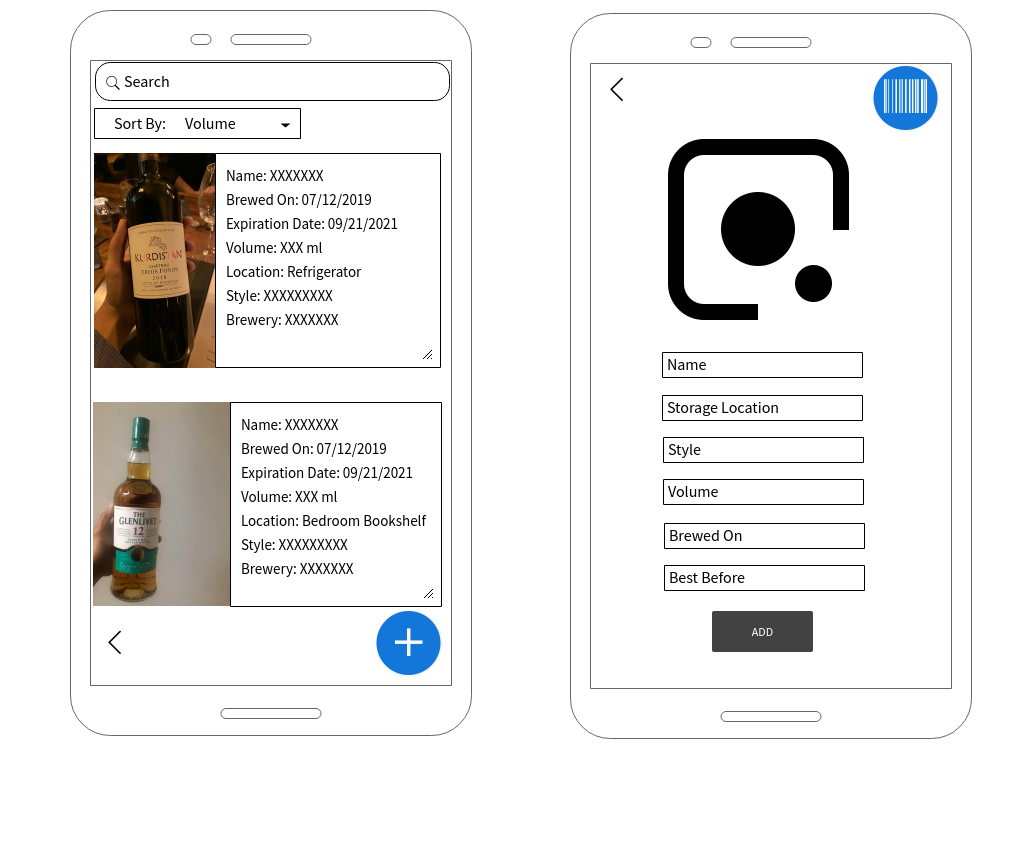
\includegraphics[width=0.60\textwidth]{images/CD.png}
    \caption{ conceptual drawing of Beverage Management App (Home screen and Add screen) }
\end{figure}

\subsection{External Inputs \& Outputs}
The users will scan the barcode of the drink, which will then access the dataset and output the details of the drink within the required storage area on the app.
Our app will extract the information as well, such as expiry date, and use it to send push notifications to the user.

\subsection{Product Interfaces}
We will have a default home screen which will display be modeled to copy Dr. Conly's storage area, in the initial release. There 
will be a button to access the camera and a settings page and an editing page as well.

\begin{figure}[h!]
	\centering
   	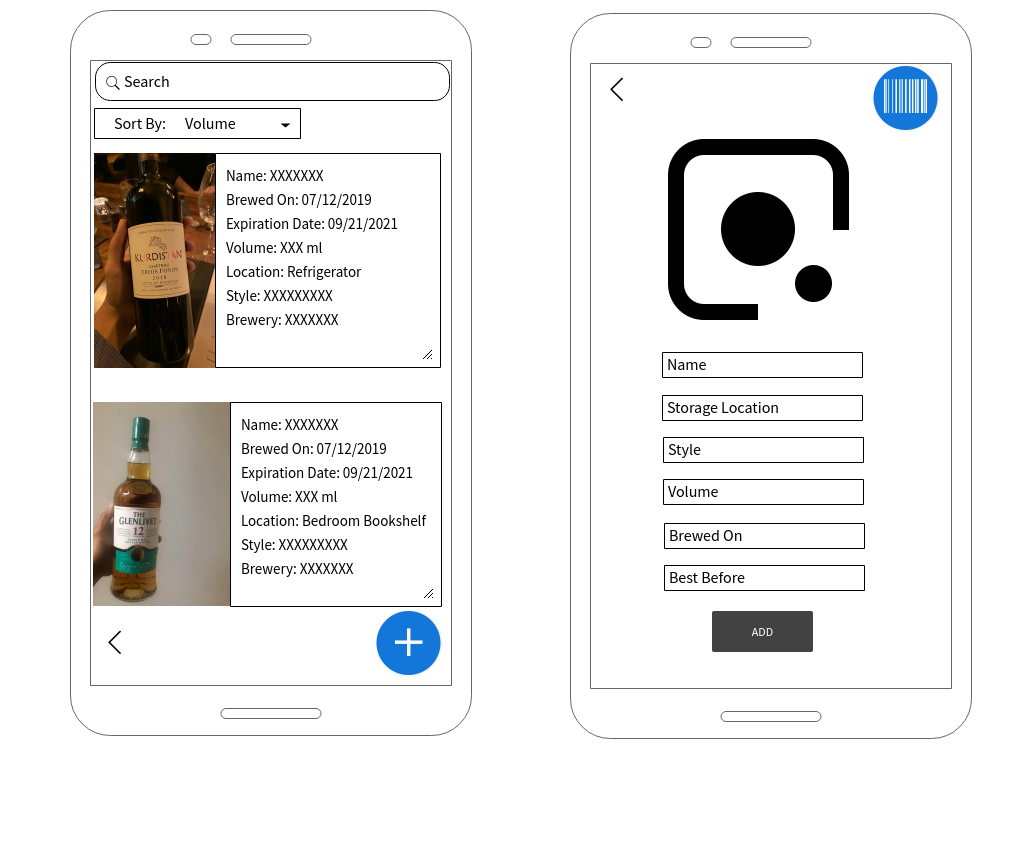
\includegraphics[width=0.60\textwidth]{images/CD.png}
    \caption{ conceptual drawing of Beverage Management App (Home screen and Add screen) }
\end{figure}